\documentclass{sigchi}

% Use this section to set the ACM copyright statement (e.g. for preprints).
% Consult the conference website for the camera-ready copyright statement.

% Copyright
\CopyrightYear{2016}
%\setcopyright{acmcopyright}
\setcopyright{acmlicensed}
%\setcopyright{rightsretained} \setcopyright{usgov} \setcopyright{usgovmixed}
%\setcopyright{cagov} \setcopyright{cagovmixed} DOI
\doi{http://dx.doi.org/10.475/123_4}
% ISBN
\isbn{123-4567-24-567/08/06}
%Conference
\conferenceinfo{CHI'16,}{May 07--12, 2016, San Jose, CA, USA}
%Price
\acmPrice{\$15.00}

% Use this command to override the default ACM copyright statement (e.g. for
% preprints).  Consult the conference website for the camera-ready copyright
% statement.

%% HOW TO OVERRIDE THE DEFAULT COPYRIGHT STRIP -- % Please note you need to make
%sure the copy for your specific % license is used here!  \toappear{ Permission
%to make digital or hard copies of all or part of this work for personal or
%classroom use is granted without fee provided that copies are not made or
%distributed for profit or commercial advantage and that copies bear this notice
%and the full citation on the first page. Copyrights for components of this work
%owned by others than ACM must be honored. Abstracting with credit is permitted.
%To copy otherwise, or republish, to post on servers or to redistribute to
%lists, requires prior specific permission and/or a fee. Request permissions
%from \href{mailto:Permissions@acm.org}{Permissions@acm.org}. \\ \emph{CHI '16},
%May 07--12, 2016, San Jose, CA, USA \\ ACM xxx-x-xxxx-xxxx-x/xx/xx\ldots
%\$15.00 \\ DOI: \url{http://dx.doi.org/xx.xxxx/xxxxxxx.xxxxxxx} }

% Arabic page numbers for submission.  Remove this line to eliminate page
% numbers for the camera ready copy \pagenumbering{arabic}

% Load basic packages
\usepackage{balance}       % to better equalize the last page
\usepackage{graphics}      % for EPS, load graphicx instead
\usepackage[T1]{fontenc}   % for umlauts and other diaeresis
\usepackage{txfonts} \usepackage{mathptmx}
\usepackage[pdflang={en-US},pdftex]{hyperref} \usepackage{color}
\usepackage{booktabs} \usepackage{textcomp}

% Some optional stuff you might like/need.
\usepackage{microtype}        % Improved Tracking and Kerning
% \usepackage[all]{hypcap}    % Fixes bug in hyperref caption linking
\usepackage{ccicons}          % Cite your images correctly!
% \usepackage[utf8]{inputenc} % for a UTF8 editor only

% If you want to use todo notes, marginpars etc. during creation of your draft
% document, you have to enable the "chi_draft" option for the document class. To
% do this, change the very first line to: "\documentclass[chi_draft]{sigchi}".
% You can then place todo notes by using the "\todo{...}"  command. Make sure to
% disable the draft option again before submitting your final document.
\usepackage{todonotes}

% Paper metadata (use plain text, for PDF inclusion and later re-using, if
% desired).  Use \emtpyauthor when submitting for review so you remain
% anonymous.
\def\plaintitle{SIGCHI Conference Proceedings Format} \def\plainauthor{First
Author, Second Author, Third Author, Fourth Author, Fifth Author, Sixth Author}
\def\emptyauthor{} \def\plainkeywords{Sketch Recognition; Gesture Recognition;
HCI} \def\plaingeneralterms{Documentation, Standardization}

% llt: Define a global style for URLs, rather that the default one
\makeatletter \def\url@leostyle{% \@ifundefined{selectfont}{ \def\UrlFont{\sf}
}{ \def\UrlFont{\small\bf\ttfamily} }} \makeatother \urlstyle{leo}

% To make various LaTeX processors do the right thing with page size.
\def\pprw{8.5in} \def\pprh{11in} \special{papersize=\pprw,\pprh}
\setlength{\paperwidth}{\pprw} \setlength{\paperheight}{\pprh}
\setlength{\pdfpagewidth}{\pprw} \setlength{\pdfpageheight}{\pprh}

% Make sure hyperref comes last of your loaded packages, to give it a fighting
% chance of not being over-written, since its job is to redefine many LaTeX
% commands.
\definecolor{linkColor}{RGB}{6,125,233} \hypersetup{% pdftitle={\plaintitle},
% Use \plainauthor for final version.  pdfauthor={\plainauthor},
  pdfauthor={\emptyauthor}, pdfkeywords={\plainkeywords},
  pdfdisplaydoctitle=true, % For Accessibility bookmarksnumbered,
  pdfstartview={FitH}, colorlinks, citecolor=black, filecolor=black,
  linkcolor=black, urlcolor=linkColor, breaklinks=true, hypertexnames=false }

% create a shortcut to typeset table headings
% \newcommand\tabhead[1]{\small\textbf{#1}}

% End of preamble. Here it comes the document.
\begin{document}

\title{\plaintitle}

\numberofauthors{3} \author{% \alignauthor{Leave Authors Anonymous\\
\affaddr{for Submission}\\ \affaddr{City, Country}\\ \email{e-mail address}}\\
\alignauthor{Leave Authors Anonymous\\ \affaddr{for Submission}\\ \affaddr{City,
Country}\\ \email{e-mail address}}\\ \alignauthor{Leave Authors Anonymous\\
\affaddr{for Submission}\\ \affaddr{City, Country}\\ \email{e-mail address}}\\ }

\maketitle

\begin{abstract} UPDATED---\today. Human emotion detection has been a wide area
of research for a very long time.  Different ways to detect humans have been
researched. Detecting expressions from static images has been done using
different classifiers such as Neural Networks or SVMs. Detecting expression from
video poses more challenges such as evaluating each frame in real time and
figuring out the emotion. In this work we present a method to detect human
facial expressions using the Microsoft Kinect 2. We utilize the FaceHD and
FaceBasics data from the kinect to classify expressions and display an emoji
accordingly. We present our results in classifying 8 different emojis. We use a
gesture based approach to classify the emotions.  Each gesture is then mapped to
a particular emoji as shown in the results.
  
\end{abstract}

\category{H.5.m.}{Information Interfaces and Presentation (e.g.
HCI)}{Miscellaneous} \category{See \url{http://acm.org/about/class/1998/} for
the full list of ACM classifiers. This section is required.}{}{}

\keywords{\plainkeywords}

\section{Introduction}

Human emotion detection and classification is a big area of research and
definitely has applications in various fields especially Human Computer
Interaction. We now have devices such as Google assistant and Amazon echo that
are capable of interacting with human beings. However, they don't take into
account sentiments or emotions. Emotions play a vital role in communication for
humans.  Charles Darwin was one of the first scientists to recognize that facial
expression is one of the most powerful and immediate means for human beings to
communicate their emotions, intentions, and opinions to each other
\cite{bartlett2003real}. As we make more and more advances in developing devices
that interact with human beings, we would need to come up with ways for
efficiently detecting and making sense of facial emotions. 

Another area of application can be MOOCs. A MOOC is a Massive Open Online
Course. MOOCs have gained immense popularity over the past few years due to the
advancement and development of online video sharing sites such as YouTube. The
classroom of the future could be set up online where students would attend
lectures by watching videos at their convenience. The system can then track the
emotions and expressions of the students and automatically figure out when the
student feels anxious about the material or when the student seems
disinterested. Based on this detection that system can improvise to provide a
better learning environment for the students.

In this paper we used the Microsoft Kinect 2 to get facial data and use that
data to classify human emotions. We then display the related emoji to that
expression. 


\section{Related Work} In this section we will talk about the related work that
has been done in this area. 

\section{Problem Statement and Overview} $Problem Statement:$ Given a set of
points from the face over a period of 20 to 30 frames, generate a gesture based
emoji recognition tool. Use the Kinect 2 FaceHD data to generate gestures and
map the correct emoji to the gestures.

The Kinect 2 has data sources: FaceHD and FaceBasics. FaceHD provides 




\begin{figure} \centering

\includegraphics[width=0.9\columnwidth]{figures/sigchi-logo} \caption{Insert a
caption below each figure. Do not alter the Caption style.  One-line captions
should be centered; multi-line should be justified. }~\label{fig:figure1}
\end{figure}

\subsection{References and Citations}



% Use a numbered list of references at the end of the article, ordered
% alphabetically by first author, and referenced by numbers in
% brackets~\cite{ethics, Klemmer:2002:WSC:503376.503378, Mather:2000:MUT,
% Zellweger:2001:FAO:504216.504224}. For papers from conference proceedings,
% include the title of the paper and an abbreviated name of the conference
% (e.g., for Interact 2003 proceedings, use \textit{Proc. Interact 2003}). Do
% not include the location of the conference or the exact date; do include the
% page numbers if available. See the examples of citations at the end of this
% document. Within this template file, use the \texttt{References} style for the
% text of your citation.

% Your references should be published materials accessible to the public.
% Internal technical reports may be cited only if they are easily accessible
% (i.e., you provide the address for obtaining the report within your citation)
% and may be obtained by any reader for a nominal fee.  Proprietary information
% may not be cited. Private communications should be acknowledged in the main
% text, not referenced (e.g., ``[Robertson, personal communication]'').

\begin{table} \centering \begin{tabular}{l r r r}
    % \toprule
    & & \multicolumn{2}{c}{\small{\textbf{Test Conditions}}} \\
    \cmidrule(r){3-4} {\small\textit{Name}} & {\small \textit{First}} & {\small
    \textit{Second}} & {\small \textit{Final}} \\ \midrule Marsden & 223.0 & 44
    & 432,321 \\ Nass & 22.2 & 16 & 234,333 \\ Borriello & 22.9 & 11 & 93,123 \\
    Karat & 34.9 & 2200 & 103,322 \\
    % \bottomrule
  \end{tabular} \caption{Table captions should be placed below the table. We
  recommend table lines be 1 point, 25\% black. Minimize use of table grid
  lines.}~\label{tab:table1} \end{table}

\begin{figure*} \centering 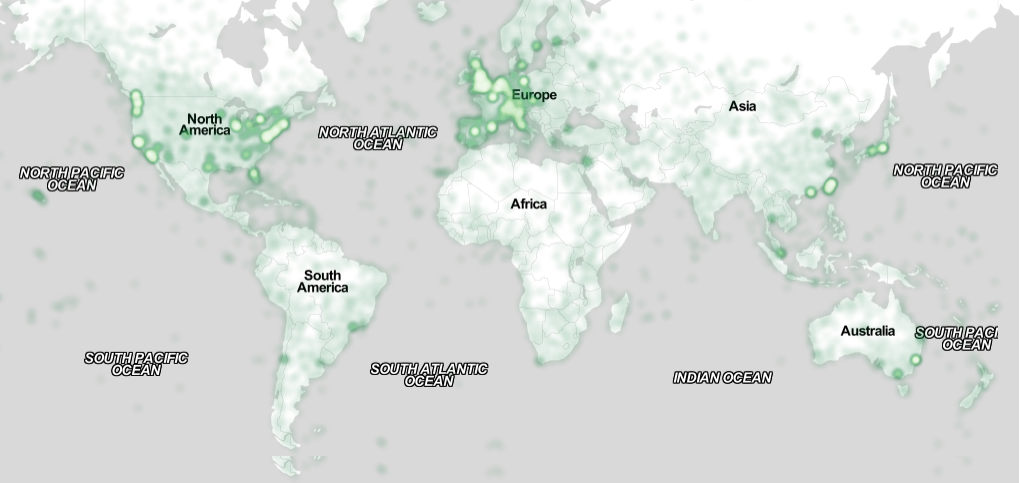
\includegraphics[width=1.75\columnwidth]{figures/map}
\caption{In this image, the map maximizes use of space. You can make figures as
wide as you need, up to a maximum of the full width of both columns. Note that
\LaTeX\ tends to render large figures on a dedicated page. Image: \ccbynd~ayman
on Flickr.}~\label{fig:figure2} \end{figure*}



\begin{itemize} \item Write in a straightforward style.  \item Try to avoid long
or complex sentence structures.  \item Briefly define or explain all technical
terms that may be unfamiliar to readers.  \item Explain all acronyms the first
time they are used in your text---e.g., ``Digital Signal Processing (DSP)''.
\item Explain local references (e.g., not everyone knows all city names in a
particular country).  \item Explain ``insider'' comments. Ensure that your whole
audience understands any reference whose meaning you do not describe (e.g., do
not assume that everyone has used a Macintosh or a particular application).
\item Explain colloquial language and puns. Understanding phrases like ``red
herring'' may require a local knowledge of English.  Humor and irony are
difficult to translate.  \item Use unambiguous forms for culturally localized
concepts, such as times, dates, currencies, and numbers (e.g., ``1--5--97'' or
``5/1/97'' may mean 5 January or 1 May, and ``seven o'clock'' may mean 7:00 am
or 19:00). For currencies, indicate equivalences: ``Participants were paid
{\fontfamily{txr}\selectfont \textwon} 25,000, or roughly US \$22.'' \item Be
careful with the use of gender-specific pronouns (he, she) and other gendered
words (chairman, manpower, man-months). Use inclusive language that is
gender-neutral (e.g., she or he, they, s/he, chair, staff, staff-hours,
person-years). See the \textit{Guidelines for Bias-Free Writing} for further
advice and examples regarding gender and other personal
attributes~\cite{Schwartz:1995:GBF}. Be particularly aware of considerations
around writing about people with disabilities.  \item If possible, use the full
(extended) alphabetic character set for names of persons, institutions, and
places (e.g., Gr{\o}nb{\ae}k, Lafreni\'ere, S\'anchez, Nguy{\~{\^{e}}}n,
Universit{\"a}t, Wei{\ss}enbach, Z{\"u}llighoven, \r{A}rhus, etc.).  These
characters are already included in most versions and variants of Times,
Helvetica, and Arial fonts.  \end{itemize}

\begin{enumerate} \item Add alternative text to all figures \item Mark table
headings \item Add tags to the PDF \item Verify the default language \item Set
the tab order to ``Use Document Structure'' \end{enumerate}

% BALANCE COLUMNS
\balance{}

% REFERENCES FORMAT References must be the same font size as other body text.
\bibliographystyle{SIGCHI-Reference-Format} \bibliography{sample}

\end{document}

%%% Local Variables: %% mode: latex %% TeX-master: t %% End:
